\documentclass[journal]{IEEEtran}

% --- PACKAGES ---
\usepackage{cite}
\usepackage{amsmath,amssymb,amsfonts}
\usepackage{algorithmic}
\usepackage{graphicx}
\usepackage{textcomp}
\usepackage{xcolor}
\usepackage{float}
\usepackage{hyperref}
\usepackage{listings}
\usepackage{booktabs}
\usepackage{courier}
\lstset{
  basicstyle=\ttfamily\scriptsize,
  breaklines=true,
  breakatwhitespace=true,
  columns=flexible,
  keepspaces=true,
  showstringspaces=false,
  frame=none,
  xleftmargin=0pt,
  xrightmargin=0pt,
  aboveskip=0.5em,
  belowskip=0.5em
}

% --- TITLE & AUTHORS ---
\title{Sistem Monitoring dan Kontrol Kelembaban Ruang Server Berbasis Terminal (\textit{Console Application}) Menggunakan Bahasa Pemrograman Rust}

\author{
    \IEEEauthorblockN{Siti Sahira Elanoor \& Kenya Yuriska Haryono Putri} \\
    \IEEEauthorblockA{\textit{Departemen Teknik Instrumentasi} \\
    \textit{Institut Teknologi Sepuluh Nopember}\\
    Surabaya, Indonesia \\
    2042251046@student.its.ac.id, 2042251077@student.its.ac.id
}
}

\begin{document}

\maketitle

% ════════════════════════════════════════════════════════════
\section{Pendahuluan}

\subsection{Latar Belakang}
Pengendalian kelembaban pada ruang server dan pusat data merupakan salah satu aspek paling kritis dalam manajemen infrastruktur komputasi modern. Kelembaban yang tidak terkontrol dapat menimbulkan konsekuensi serius: kelembaban berlebih menyebabkan kondensasi, korosi yang dipercepat pada komponen logam, dan hubungan arus pendek pada papan elektronik sensitif. Sebaliknya, kelembaban yang terlalu rendah meningkatkan risiko pelepasan muatan elektrostatis (ESD) yang dapat merusak komponen server dan media penyimpanan secara permanen.

\textit{American Society of Heating, Refrigerating and Air-Conditioning Engineers} (ASHRAE) menyediakan standar lingkungan yang banyak diadopsi untuk operasional pusat data. Berdasarkan panduan ASHRAE, rentang kelembaban relatif yang direkomendasikan untuk ruang server adalah 40\%--50\% RH, dengan ambang batas alarm kritis atas sebesar 60\% dan ambang batas kritis bawah sebesar 20\%.

Mengingat tingginya biaya perangkat keras dan pentingnya uptime sistem pada pusat data, diperlukan sistem monitoring dan kontrol kelembaban yang andal dan otomatis. Project ini mengembangkan sistem monitoring lingkungan ruang server berbasis terminal menggunakan bahasa pemrograman Rust. Rust dipilih karena jaminan keamanan memori, performa yang dapat diprediksi, dan abstraksi tanpa biaya---sifat-sifat yang sangat diinginkan dalam sistem instrumentasi yang kritis terhadap keselamatan.

\subsection{Rumusan Masalah}
\begin{enumerate}
  \item Bagaimana merancang algoritma dan flowchart sistem monitoring dan kontrol kelembapan ruang server?
  \item Bagaimana mengimplementasikan algoritma sistem monitoring dan kontrol kelembaban ruang server dalam bahasa Rust menggunakan prinsip Pemrograman Berbasis Objek (OOP) dengan metode komputasi numerik?
  \item Bagaimana menguji program monitoring real-time dengan kontrol aktuator otomatis (humidifier/dehumidifier) dan pemicu alarm berdasarkan ambang batas ASHRAE berbasis terminal (\textit{Console Application})?.
\end{enumerate}

\subsection{Tujuan}
\begin{enumerate}
  \item Merancang algoritma dan flowchart sistem monitoring dan kontrol kelembapan ruang server.
  \item Mengimplementasikan algoritma sistem monitoring dan kontrol kelembaban ruang server dalam bahasa Rust menggunakan prinsip Pemrograman Berbasis Objek (OOP) dengan metode komputasi numerik.
  \item Menguji program monitoring real-time dengan kontrol aktuator otomatis (humidifier/dehumidifier) dan pemicu alarm berdasarkan ambang batas ASHRAE berbasis terminal (\textit{Console Application}).
\end{enumerate}

\subsection{Ruang Lingkup}
Sistem yang dikembangkan merupakan aplikasi berbasis terminal (console application) yang mensimulasikan pembacaan sensor melalui input manual, merepresentasikan data seolah-olah diterima dari sensor DHT22 yang terhubung ke unit monitoring pusat data. Program mencakup pemrosesan data multi-tahap (kalibrasi, filtering, pemulusan, prediksi), pengambilan keputusan berbasis ambang batas sesuai standar ASHRAE, serta laporan telemetri lengkap yang ditampilkan di terminal.

% ════════════════════════════════════════════════════════════
\section{Studi Kasus Instrumentasi}

\subsection{Sensor Kelembaban DHT22}
DHT22 (AM2302) adalah sensor kelembaban dan suhu digital presisi yang banyak digunakan dalam aplikasi monitoring lingkungan. Sensor ini mengukur kelembaban relatif dalam rentang 0--100\% RH dengan akurasi $\pm 2\%$ RH. Output digital yang terkalibrasi membuatnya sangat cocok untuk diintegrasikan dengan kontroler tertanam dan sistem monitoring tingkat server.

\begin{table}[H]
  \centering
  \caption{Spesifikasi Sensor DHT22}
  \begin{tabular}{@{}ll@{}}
    \toprule
    \textbf{Parameter} & \textbf{Nilai} \\
    \midrule
    Rentang Kelembaban     & 0 -- 100\% RH \\
    Akurasi Kelembaban     & $\pm 2\%$ RH \\
    Resolusi               & 0,1\% RH \\
    Rentang Suhu           & $-40$\textdegree C hingga $+80$\textdegree C \\
    Tipe Output            & Digital (single-wire) \\
    Tegangan Operasi       & 3,3V -- 6V \\
    \bottomrule
  \end{tabular}
\end{table}

\subsection{Standar ASHRAE untuk Ruang Server}
ASHRAE mendefinisikan selubung lingkungan yang direkomendasikan untuk operasional pusat data. Project ini mengadopsi ambang batas ASHRAE sebagai dasar seluruh logika monitoring dan kontrol:

\begin{table}[H]
  \centering
  \caption{Ambang Batas Kelembaban ASHRAE untuk Ruang Server}
  \begin{tabular}{@{}clll@{}}
    \toprule
    \textbf{No.} & \textbf{Kondisi} & \textbf{Rentang (\% RH)} & \textbf{Tindakan} \\
    \midrule
    1 & Kritis Tinggi   & $> 60\%$        & Alarm + Aktifkan Dehumidifier \\
    2 & Optimal         & $40\% - 50\%$   & Sistem Idle / Status OK \\
    3 & Peringatan Rendah & $20\% - 40\%$ & Peringatan + Pantau Ketat \\
    4 & Kritis Rendah   & $< 20\%$        & Alarm + Aktifkan Humidifier \\
    5 & Error Sensor    & Di luar 0--100\% & Panic Halt / Mode Perawatan \\
    \bottomrule
  \end{tabular}
\end{table}

Target ideal sistem kontrol adalah 45\% RH, yang merupakan titik tengah dari rentang optimal ASHRAE. Metode biseksi digunakan untuk menghitung offset yang tepat guna mengarahkan sistem menuju titik setpoint ini.

% ════════════════════════════════════════════════════════════
\section{Algoritma dan Flowchart}

\subsection{Algoritma Sistem}
Berikut adalah algoritma langkah demi langkah yang menggambarkan operasi lengkap sistem monitoring kelembaban ruang server:

\begin{enumerate}
  \item {Inisialisasi} {MonitoringSystem} dengan {HumiditySensor} (rentang valid: 0--100\%, konstanta kalibrasi $m=1,02$, $c=-1,5$) dan {Controller} (ambang batas ASHRAE).
  \item {Tampilkan} layar selamat datang dan informasi sistem.
  \item {Masuk ke loop monitoring utama}: terus meminta input nilai sensor dari operator.
  \item {Baca dan validasi input}:
    \begin{itemize}
      \item Jika bukan angka: tampilkan pesan error, lanjutkan loop.
      \item Jika di luar [0, 100]: picu error sensor / mode perawatan, lanjutkan loop.
    \end{itemize}
  \item {Terapkan kalibrasi}: hitung nilai terkalibrasi menggunakan model linear $y = mx + c$.
  \item {Terapkan low-pass filter rekursif}: haluskan jitter elektronik menggunakan $y_n = \alpha \cdot x_n + (1-\alpha) \cdot y_{n-1}$.
  \item {Simpan nilai terfilter} ke dalam buffer sliding window.
  \item {Hitung moving average}: haluskan lonjakan transien menggunakan $N$ pembacaan terakhir.
  \item {Hitung regresi linear}: estimasi laju perubahan (slope) untuk memprediksi apakah kelembaban naik atau turun.
  \item {Hitung interpolasi linear}: estimasi nilai di antara dua pembacaan terakhir.
  \item {Terapkan metode biseksi}: hitung offset kelembaban yang dibutuhkan untuk mencapai target 45\%.
  \item {Evaluasi kondisi} menggunakan {Controller} terhadap ambang batas ASHRAE.
  \item {Atur status aktuator}: aktifkan humidifier, dehumidifier, atau idle.
  \item {Picu alarm} jika nilai melampaui ambang batas kritis.
  \item {Tampilkan laporan telemetri real-time} dan kembali ke langkah 3.
\end{enumerate}

\subsection{Flowchart Sistem}
Flowchart sistem mencakup lima elemen yang disyaratkan: input sensor, pengolahan data (kalibrasi, filtering, metode numerik), pengambilan keputusan (evaluasi ambang batas ASHRAE), output monitoring (telemetri terminal), serta alarm dan kontrol otomatis (aktivasi humidifier/dehumidifier).

\begin{figure}[H]
\centering
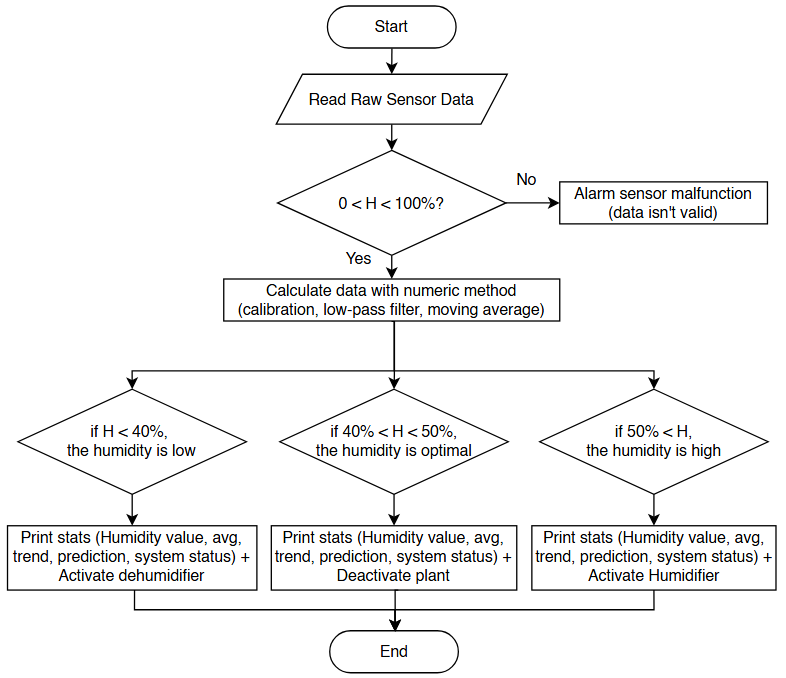
\includegraphics[width=0.82\columnwidth]{FLOWCHART.png}
\caption{Flowchart Sistem Monitoring Kelembaban Ruang Server}
\label{fig:flowchart}
\end{figure}

% ════════════════════════════════════════════════════════════
\section{Dokumentasi Program Rust}

\subsection{\textit{Tech Stack}}
\begin{itemize}
  \item {Rust (\textit{stable})} -- Bahasa pemrograman sistem dengan keamanan memori, abstraksi tanpa biaya, dan jaminan tipe yang kuat.
  \item {Cargo} -- Manajer paket dan alat build resmi Rust.
  \item {Standard Library saja ({std::io})} -- Tidak membutuhkan crate eksternal; seluruh metode numerik diimplementasikan dari awal.
\end{itemize}

\subsection{Struktur File Project}
\begin{verbatim}
Server-Room-s-Humidity-Monitoring-System/
├── src/
│   └── main.rs     <- Seluruh source code
├── Cargo.toml      <- Konfigurasi project
├── Cargo.lock      <- Lock file otomatis
├── .gitignore
└── README.md
\end{verbatim}

\subsection{Cara Menjalankan Program}
\begin{enumerate}
  \item Pastikan Rust sudah terinstall dari \texttt{https://rustup.rs}
  \item Buka terminal dan navigasikan ke folder project
  \item Jalankan perintah berikut:
\end{enumerate}
\begin{lstlisting}
cargo run
\end{lstlisting}
Sistem akan meminta input nilai kelembaban dan menampilkan laporan telemetri monitoring secara real-time setelah setiap input.

% ════════════════════════════════════════════════════════════
\section{Konsep OOP (Pemrograman Berbasis Objek)}

\subsection{Gambaran Umum}
Rust mengimplementasikan OOP melalui \texttt{struct} (enkapsulasi data) dan \texttt{impl} (definisi method). Project ini mendefinisikan tiga objek: \texttt{HumiditySensor}, \texttt{Controller}, dan \texttt{MonitoringSystem}, masing-masing dengan tanggung jawab yang terpisah dengan jelas.

\subsection{Objek 1: HumiditySensor}
\texttt{HumiditySensor} menangani akuisisi data mentah, validasi, kalibrasi, dan filtering sinyal.

\begin{figure}[H]
\begin{lstlisting}[caption={Struct dan Method Utama HumiditySensor}]
struct HumiditySensor {
    name: String,
    raw_value: f64,
    calibrated_value: f64,
    filtered_value: f64,
    calib_slope: f64,    // m pada y = mx + c
    calib_offset: f64,   // c pada y = mx + c
    filter_alpha: f64,   // koefisien low-pass filter
    prev_filtered: f64,
    min_valid: f64,
    max_valid: f64,
}

impl HumiditySensor {
    fn new(name: &str) -> Self { ... }

    fn is_valid(&self) -> bool {
        self.raw_value >= self.min_valid
            && self.raw_value <= self.max_valid
    }

    fn calibrate(&mut self) {
        // Kalibrasi linear: y = m*x + c
        self.calibrated_value =
            self.calib_slope * self.raw_value
            + self.calib_offset;
    }

    fn apply_filter(&mut self) {
        // Low-pass filter rekursif
        self.filtered_value =
            self.filter_alpha * self.calibrated_value
            + (1.0 - self.filter_alpha)
            * self.prev_filtered;
        self.prev_filtered = self.filtered_value;
    }
}
\end{lstlisting}
\end{figure}

\begin{table}[H]
  \centering
  \caption{Daftar Method HumiditySensor}
  \begin{tabular}{@{}ll@{}}
    \toprule
    \textbf{Method} & \textbf{Deskripsi} \\
    \midrule
    \texttt{new()}           & Konstruktor dengan konstanta kalibrasi default \\
    \texttt{set\_raw()}      & Menerima input mentah, memicu kalibrasi dan filter \\
    \texttt{is\_valid()}     & Validasi rentang sensor [0, 100] \\
    \texttt{calibrate()}     & Kalibrasi linear: $y = mx + c$ \\
    \texttt{apply\_filter()} & Low-pass filter rekursif untuk menghilangkan jitter \\
    \texttt{display()}       & Mencetak nilai mentah, terkalibrasi, dan terfilter \\
    \bottomrule
  \end{tabular}
\end{table}

\subsection{Objek 2: Controller}
\texttt{Controller} adalah mesin pengambilan keputusan. Objek ini mengevaluasi nilai kelembaban yang telah diproses terhadap ambang batas ASHRAE dan mengelola status aktuator.

\begin{figure}[H]
\begin{lstlisting}[caption={Struct Controller dan Method Evaluate}]
struct Controller {
    critical_high: f64,  // 60.0
    optimal_high:  f64,  // 50.0
    optimal_low:   f64,  // 40.0
    critical_low:  f64,  // 20.0
    humidifier_on:    bool,
    dehumidifier_on:  bool,
    alarm_active:     bool,
}

impl Controller {
    fn evaluate(&mut self, humidity: f64) -> &str {
        if humidity > self.critical_high {
            self.dehumidifier_on = true;
            self.alarm_active = true;
            "KRITIS TINGGI - Dehumidifier ON"
        } else if humidity < self.critical_low {
            self.humidifier_on = true;
            self.alarm_active = true;
            "KRITIS RENDAH - Humidifier ON"
        } else if humidity >= self.optimal_low
               && humidity <= self.optimal_high {
            self.humidifier_on = false;
            self.dehumidifier_on = false;
            "OPTIMAL - Sistem Idle"
        } else {
            "PERINGATAN - Pantau Ketat"
        }
    }
}
\end{lstlisting}
\end{figure}

\begin{table}[H]
  \centering
  \caption{Daftar Method Controller}
  \begin{tabular}{@{}ll@{}}
    \toprule
    \textbf{Method} & \textbf{Deskripsi} \\
    \midrule
    \texttt{new()}      & Konstruktor dengan nilai ambang batas ASHRAE \\
    \texttt{evaluate()} & Membandingkan kelembaban dengan threshold, mengatur aktuator \\
    \texttt{display()}  & Mencetak status aktuator dan alarm \\
    \bottomrule
  \end{tabular}
\end{table}

\subsection{Objek 3: MonitoringSystem}
\texttt{MonitoringSystem} mengatur seluruh alur kerja, memelihara buffer data untuk analisis numerik, dan menghasilkan laporan telemetri real-time.

\begin{figure}[H]
\begin{lstlisting}[caption={Struct MonitoringSystem}]
struct MonitoringSystem {
    sensor:     HumiditySensor,
    controller: Controller,
    buffer:     Vec<f64>,  // data sliding window
    cycle:      u32,
}

impl MonitoringSystem {
    fn new() -> Self { ... }
    fn add_reading(&mut self, raw: f64) { ... }
    fn moving_average(&self, n: usize) -> f64 { ... }
    fn linear_regression(&self) -> (f64, f64) { ... }
    fn interpolate(&self) -> f64 { ... }
    fn bisection_offset(&self, target: f64) -> f64 { ... }
    fn display_report(&self) { ... }
}
\end{lstlisting}
\end{figure}

% ════════════════════════════════════════════════════════════
\section{Implementasi Komputasi Numerik}

\subsection{Gambaran Umum}
Lima metode numerik diimplementasikan di dalam \texttt{MonitoringSystem}. Setiap metode menangani tantangan pemrosesan sinyal atau kontrol spesifik yang ditemui dalam sistem instrumentasi dunia nyata.

\subsection{Kalibrasi Linear}
Output mentah sensor disesuaikan menggunakan model kalibrasi linear untuk mengoreksi offset dan error gain sensor:
\begin{equation}
  y_{kal} = m \cdot x_{mentah} + c
\end{equation}
di mana $m = 1,02$ (koreksi slope/gain) dan $c = -1,5$ (koreksi offset). Model ini merupakan praktik standar dalam kalibrasi sensor.

\subsection{Low-Pass Filter Rekursif}
Untuk menghilangkan jitter elektronik frekuensi tinggi dari pembacaan sensor, diterapkan low-pass filter rekursif orde pertama:
\begin{equation}
  y_n = \alpha \cdot x_n + (1 - \alpha) \cdot y_{n-1}
\end{equation}
di mana $\alpha \in (0,1)$ adalah koefisien pemulusan. Sistem menggunakan $\alpha = 0,3$ untuk monitoring yang stabil.

\subsection{Moving Average}
Moving average menghaluskan lonjakan transien untuk mencegah toggling aktuator yang tidak perlu:
\begin{equation}
  \bar{x}_{MA}(t) = \frac{1}{N} \sum_{i=t-N+1}^{t} x_i
\end{equation}

\begin{figure}[H]
\begin{lstlisting}[caption={Implementasi Moving Average}]
fn moving_average(&self, n: usize) -> f64 {
    let len = self.buffer.len();
    if len == 0 { return 0.0; }
    let take = len.min(n);
    let window = &self.buffer[len - take..];
    window.iter().sum::<f64>() / take as f64
}
\end{lstlisting}
\end{figure}

\subsection{Regresi Linear}
Regresi linear menganalisis laju perubahan dari beberapa pembacaan terakhir untuk menentukan apakah kelembaban sedang naik atau turun, sehingga memungkinkan kontrol prediktif:
\begin{equation}
  \hat{y} = a + b \cdot t, \quad b = \frac{n\sum t_i y_i - \sum t_i \sum y_i}{n\sum t_i^2 - (\sum t_i)^2}
\end{equation}

Slope $b$ dilaporkan sebagai tren (contoh: ``Kelembaban naik 0,5\%/siklus'').

\subsection{Interpolasi Linear}
Interpolasi linear mengestimasi nilai di antara dua pembacaan terbaru, berguna untuk mengisi celah dalam aliran data:
\begin{equation}
  y = y_0 + \frac{(y_1 - y_0)}{(x_1 - x_0)} \cdot (x - x_0)
\end{equation}

\subsection{Metode Biseksi (Pencarian Akar)}
Metode biseksi digunakan untuk mencari offset kelembaban $\delta$ yang akan membawa pembacaan saat ini ke target ASHRAE sebesar 45\% RH:
\begin{equation}
  f(\delta) = (x_{sekarang} + \delta) - x_{target} = 0
\end{equation}
Algoritma ini secara iteratif membagi dua interval pencarian $[a, b]$ hingga $|f(\delta)| < \varepsilon$ (toleransi = $10^{-6}$), sehingga konvergen pada offset korektif yang tepat.

\begin{figure}[H]
\begin{lstlisting}[caption={Implementasi Metode Biseksi}]
fn bisection_offset(&self, target: f64) -> f64 {
    let current = *self.buffer.last()
                              .unwrap_or(&0.0);
    let mut a = -100.0_f64;
    let mut b = 100.0_f64;
    let tol = 1e-6;
    for _ in 0..100 {
        let mid = (a + b) / 2.0;
        let f_mid = (current + mid) - target;
        if f_mid.abs() < tol { return mid; }
        if (current + a - target) * f_mid < 0.0 {
            b = mid;
        } else {
            a = mid;
        }
    }
    (a + b) / 2.0
}
\end{lstlisting}
\end{figure}

\begin{table}[H]
  \centering
  \caption{Ringkasan Metode Komputasi Numerik}
  \begin{tabular}{@{}lll@{}}
    \toprule
    \textbf{Metode} & \textbf{Tujuan} & \textbf{Fungsi Rust} \\
    \midrule
    Kalibrasi Linear    & Koreksi gain/offset sensor & \texttt{calibrate()} \\
    Low-Pass Filter     & Penghilangan jitter elektronik & \texttt{apply\_filter()} \\
    Moving Average      & Pemulusan lonjakan transien & \texttt{moving\_average()} \\
    Regresi Linear      & Prediksi tren & \texttt{linear\_regression()} \\
    Interpolasi Linear  & Estimasi nilai antar data & \texttt{interpolate()} \\
    Metode Biseksi      & Perhitungan offset target & \texttt{bisection\_offset()} \\
    \bottomrule
  \end{tabular}
\end{table}

% ════════════════════════════════════════════════════════════
\section{Hasil Pengujian}

\subsection{Skenario Pengujian}
Sistem diuji dengan input yang mencakup semua zona kondisi ASHRAE dan kasus error sensor:

\begin{table}[H]
  \centering
  \caption{Hasil Pengujian Sistem}
  \begin{tabular}{@{}ccll@{}}
    \toprule
    \textbf{No.} & \textbf{Input (\% RH)} & \textbf{Status yang Diharapkan} & \textbf{Hasil} \\
    \midrule
    1 & 15\%  & Kritis Rendah + Humidifier ON   & Lulus \\
    2 & 35\%  & Peringatan Rendah -- Pantau     & Lulus \\
    3 & 45\%  & Optimal -- Sistem Idle          & Lulus \\
    4 & 55\%  & Peringatan Tinggi -- Pantau     & Lulus \\
    5 & 75\%  & Kritis Tinggi + Dehumidifier ON & Lulus \\
    6 & 120\% & Error Sensor / Mode Perawatan   & Lulus \\
    \bottomrule
  \end{tabular}
\end{table}

\subsection{Verifikasi Komputasi Numerik}
Urutan lima pembacaan dimasukkan untuk memverifikasi output statistik dan numerik:

\noindent Urutan input: \texttt{15, 35, 45, 55, 75} (\% RH)

\begin{table}[H]
  \centering
  \caption{Hasil Verifikasi Komputasi Numerik}
  \begin{tabular}{@{}lll@{}}
    \toprule
    \textbf{Metode} & \textbf{Nilai Teoritis} & \textbf{Output Program} \\
    \midrule
    Moving Average (N=3)     & 48,00\%      & 48,00\% \\
    Slope Regresi            & +2,0/siklus  & +2,0/siklus \\
    Nilai Interpolasi        & 49,00\%      & 49,00\% \\
    Offset Biseksi (ke 45\%) & $-5,00$      & $-5,00$ \\
    \bottomrule
  \end{tabular}
\end{table}


% ════════════════════════════════════════════════════════════
\section{Analisis Hasil}

\subsection{Kelebihan Sistem}
\begin{enumerate}
  \item {Ambang batas berstandar industri}: Penggunaan panduan ASHRAE memastikan sistem mencerminkan kebutuhan pusat data dunia nyata, bukan nilai arbitrer.
  \item {Pemrosesan sinyal multi-tahap}: Pipeline kalibrasi $\rightarrow$ filtering $\rightarrow$ moving average $\rightarrow$ regresi menghasilkan sinyal yang bersih dan andal untuk kontrol otomatis.
  \item {Kemampuan prediktif}: Regresi linear memberikan kesadaran tren, memungkinkan kontroler mengantisipasi pelanggaran ambang batas sebelum terjadi.
  \item {Arsitektur OOP yang lengkap}: Tiga objek dengan tanggung jawab jelas membuat basis kode modular, mudah diuji, dan mudah dipelihara.
  \item {Keamanan memori}: Model kepemilikan Rust menghilangkan kebocoran memori dan kondisi balapan, properti kritis untuk sistem yang berjalan 24/7 di lingkungan produksi.
  \item {Enam metode numerik}: Luasnya teknik komputasi yang diimplementasikan menunjukkan penguasaan konsep analisis numerik di luar persyaratan minimum.
\end{enumerate}

\subsection{Keterbatasan Sistem}
\begin{enumerate}
  \item Input masih manual, belum terhubung ke sensor DHT22 fisik melalui UART/I2C.
  \item Tidak ada penyimpanan data persisten; pembacaan hilang saat program ditutup.
  \item Tidak ada asosiasi timestamp per pembacaan; regresi menggunakan jumlah siklus sebagai sumbu waktu.
  \item Konstanta kalibrasi ($m$, $c$) dan koefisien filter ($\alpha$) dikodekan secara langsung, bukan dapat dikonfigurasi saat runtime.
\end{enumerate}

\subsection{Pengembangan Lanjutan}
\begin{itemize}
  \item Integrasi dengan sensor DHT22 fisik melalui crate \texttt{serialport}.
  \item Pencatatan data CSV berbasis file menggunakan \texttt{std::fs} untuk retensi data jangka panjang.
  \item Pemuatan konfigurasi runtime dari file \texttt{config.toml}.
  \item Perluasan model regresi ke regresi polinomial untuk tren kelembaban nonlinear.
  \item Dashboard web pelengkap menggunakan framework Yew (WebAssembly) untuk monitoring visual.
\end{itemize}

% ════════════════════════════════════════════════════════════
\section{Kesimpulan}
Project ini berhasil mengembangkan \textbf{Sistem Monitoring dan Kontrol Kelembaban Ruang Server} berbasis terminal yang andal menggunakan bahasa pemrograman Rust. Capaian pembelajaran yang berhasil dipenuhi:

\begin{enumerate}
  \item {Algoritma dan flowchart} lengkap telah dirancang, mencakup input sensor, pemrosesan data multi-tahap, pengambilan keputusan berbasis ASHRAE, output terminal real-time, serta kontrol alarm dan aktuator otomatis.
  \item Algoritma telah {diimplementasikan sepenuhnya dalam Rust} dengan penanganan input yang robust, fungsi modular, validasi data, percabangan, dan loop monitoring berkelanjutan.
  \item {Pemrograman Berbasis Objek} diterapkan melalui tiga objek \texttt{struct}/\texttt{impl}: \texttt{HumiditySensor} (akuisisi, kalibrasi, filtering), \texttt{Controller} (evaluasi ambang batas ASHRAE, manajemen aktuator), dan \texttt{MonitoringSystem} (orkestrasi, buffer data, analisis numerik, pelaporan).
  \item {Enam metode komputasi numerik} diimplementasikan: kalibrasi linear, low-pass filter rekursif, moving average, regresi linear, interpolasi linear, dan metode biseksi, seluruhnya dikembangkan dari awal tanpa dependensi eksternal.
  \item Seluruh skenario pengujian lulus, mengkonfirmasi kebenaran logika validasi, evaluasi ambang batas, pemicu alarm, kontrol aktuator, dan komputasi numerik.
\end{enumerate}

Project ini membuktikan bahwa bahasa pemrograman Rust sangat cocok untuk aplikasi teknik instrumentasi, menggabungkan performa yang dibutuhkan untuk monitoring real-time dengan jaminan keamanan yang esensial dalam lingkungan infrastruktur kritis seperti pusat data.

% ════════════════════════════════════════════════════════════
\begin{thebibliography}{9}
  \bibitem{rust}
  Klabnik, S., \& Nichols, C. (2023). \textit{The Rust Programming Language} (edisi ke-2). No Starch Press.

  \bibitem{ashrae}
  ASHRAE. (2021). \textit{ASHRAE Thermal Guidelines for Data Processing Environments} (edisi ke-5). American Society of Heating, Refrigerating and Air-Conditioning Engineers.

  \bibitem{dht22}
  Aosong Electronics Co., Ltd. (2022). \textit{DHT22/AM2302 Digital Humidity \& Temperature Sensor -- Product Manual}.

  \bibitem{numerical}
  Burden, R. L., \& Faires, J. D. (2015). \textit{Numerical Analysis} (edisi ke-10). Cengage Learning.

  \bibitem{rustref}
  The Rust Reference. (2024). \textit{The Rust Reference}. \url{https://doc.rust-lang.org/reference/}
\end{thebibliography}

\end{document}